%   Filename    : chapter_4.tex 
\chapter{Research Methodology}
This chapter lists and discusses the specific steps and activities that will be performed to accomplish the project. 
The discussion covers the activities from pre-proposal to Final SP Writing.

\begin{figure}[ht]
	\centering
	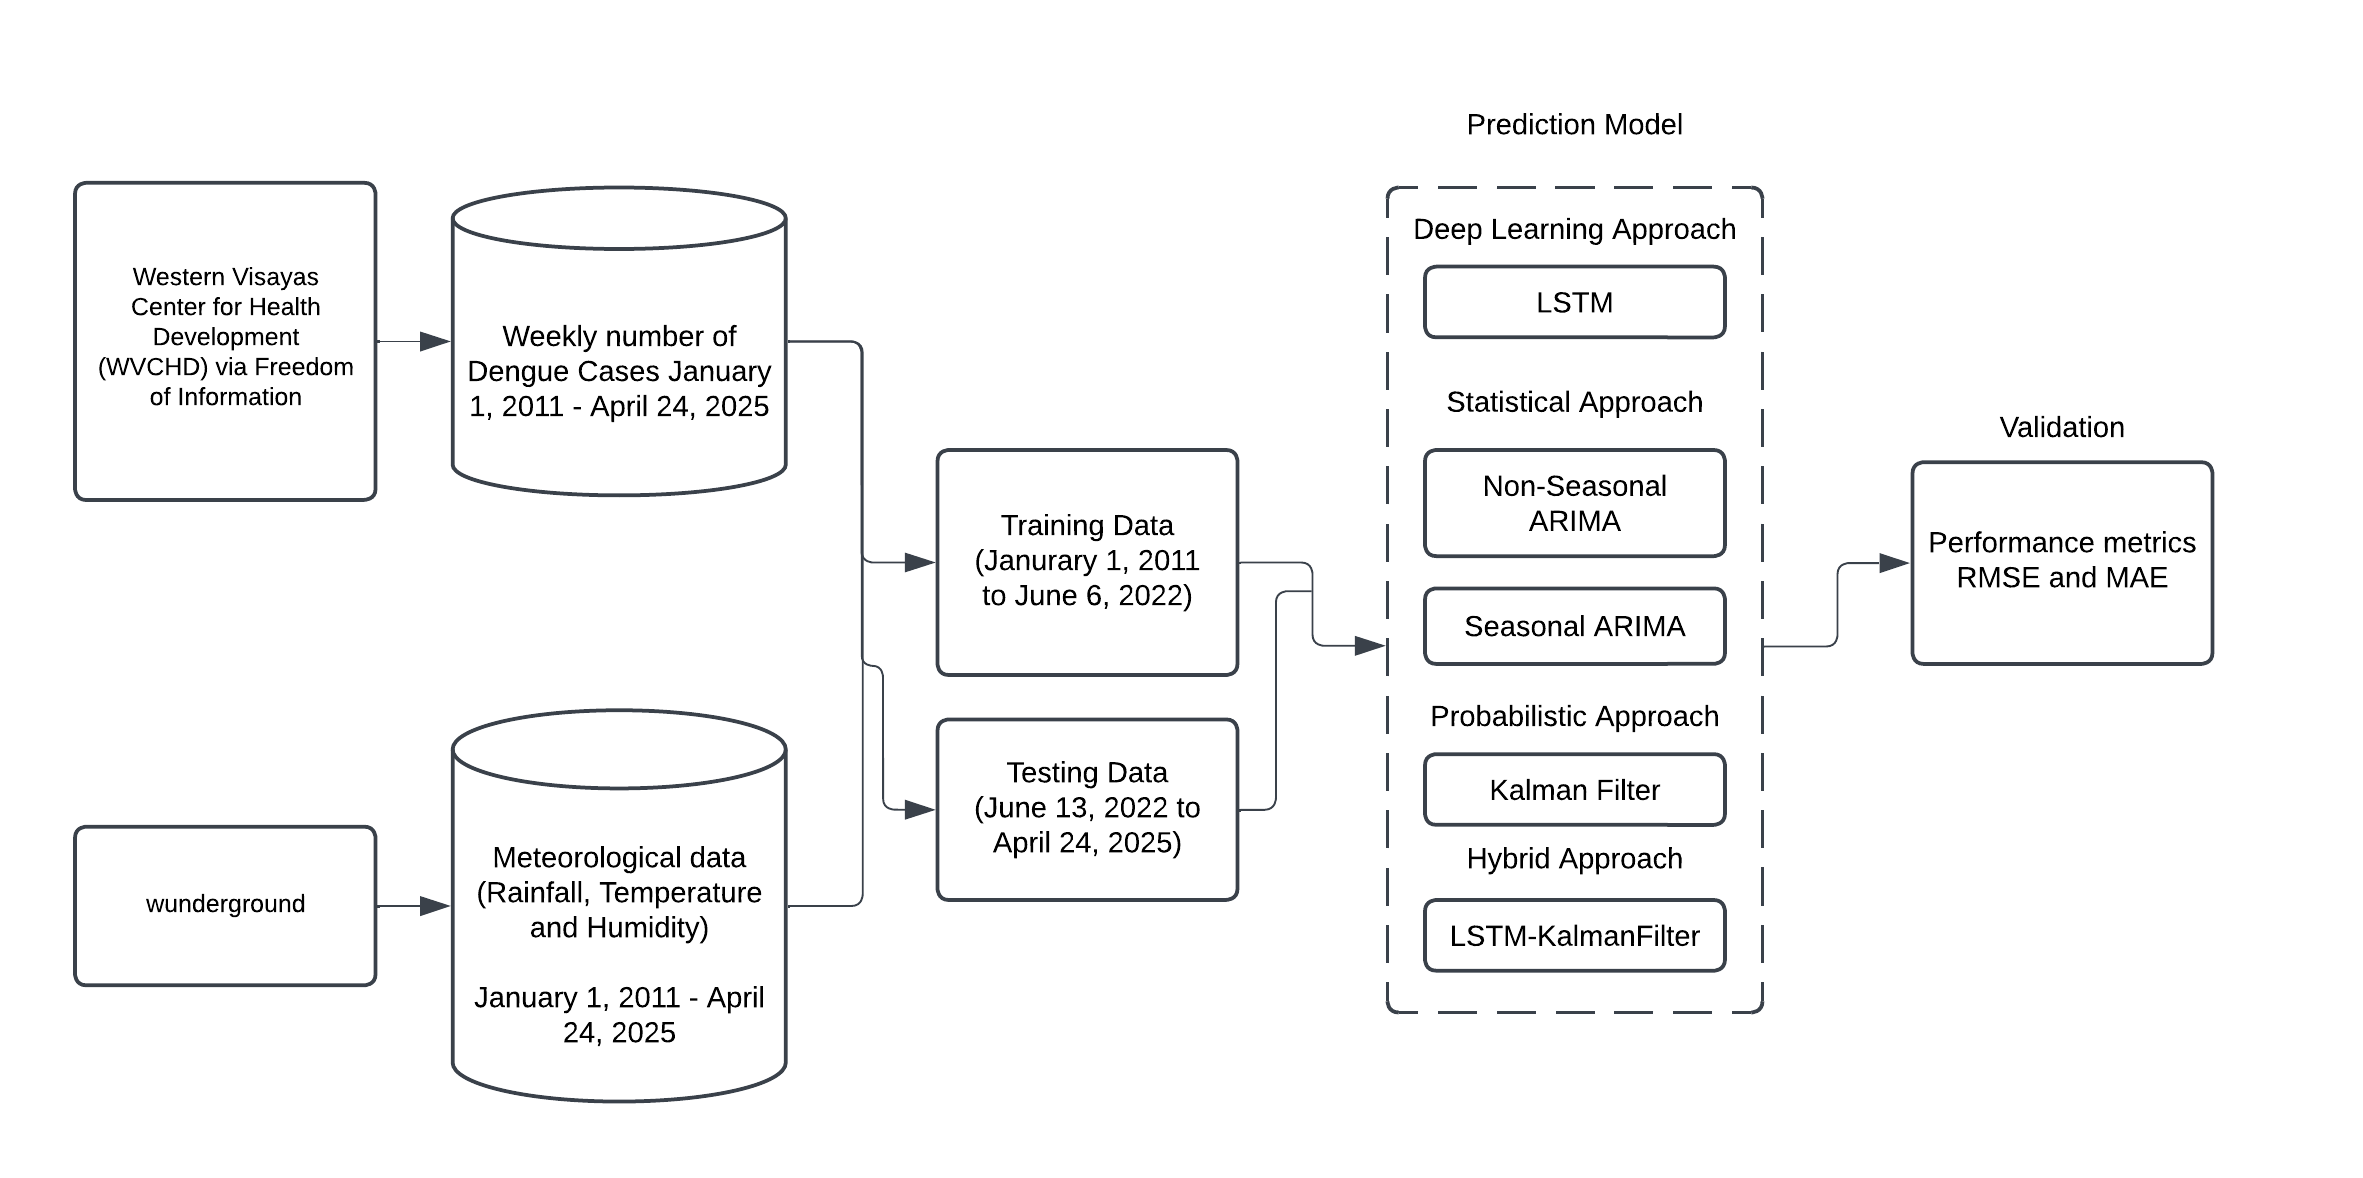
\includegraphics[width=0.75\textwidth]{Model Diagram}
	\caption{Workflow for forecasting the number of weekly dengue cases}
	\label{fig:data_snippet}
\end{figure}
This summarizes the workflow for forecasting the number of weekly dengue cases. This workflow focuses on using statistical, deep learning, and probabilistic models to forecast the number of reported dengue cases. The approach involves deploying several models for prediction, including ARIMA and Seasonal ARIMA as statistical approaches, LSTM as a deep learning approach, and the Kalman Filter as a probabilistic approach. These methods are compared with each other to determine the most accurate model.
\section{Research Activities}

\subsection{Gather Dengue Data and Climate Data to Create a Complete Dataset for Forecasting}

\subsubsection{Acquisition of Dengue Case Data}
The historical dengue case dataset used in this study was obtained from the Humanitarian Data Exchange and the Western Visayas Center for Health Development (WVCHD) via Freedom of Information (FOI) requests. The decision to use weekly intervals was driven by the need for precision and timeliness in capturing fluctuations in dengue cases and weather conditions. Dengue transmission is influenced by short-term changes in weather variables such as rainfall and temperature, which impact mosquito breeding and virus transmission cycles. A weekly granularity allowed the model to better capture these short-term trends, enabling more accurate predictions and responsive public health interventions.

Moreover, using a weekly interval provided more data points for training the models compared to a monthly format. This is particularly critical in time series modeling, where larger datasets help improve the robustness of the model and its ability to generalize to new data. Also, the collection of weather data was done by utilizing web scraping techniques to extract weekly weather data (e.g., rainfall, temperature, and humidity) from Weather Underground (wunderground.com).
\\
\\
\textbf{Data Fields}
\begin{itemize}
	\item \textbf{Time.} Represents the specific year and week corresponding to each entry in the dataset.
	\item \textbf{Rainfall.} Denotes the observed average rainfall, measured in millimeters, for a specific week.
	\item \textbf{Humidity.} Refers to the observed average relative humidity, expressed as a percentage, for a specific week.    
	\item \textbf{Max Temperature.} Represents the observed maximum temperature, measured in degrees Celsius, for a specific week.
	\item \textbf{Average Temperature.} Represents the observed average temperature, measured in degrees Celsius, for a specific week.
	\item \textbf{Min Temperature.} Represents the observed minimum temperature, measured in degrees Celsius, for a specific week.
	\item \textbf{Wind.} Represents the observed wind speed, measured in miles per hour (mph), for a specific week.
	\item \textbf{Cases.} Refers to the number of reported dengue cases during a specific week.
\end{itemize} 

\subsubsection{Data Integration and Preprocessing}
The dengue case data was integrated with the weather data to create a com
prehensive dataset, aligning the data based on corresponding timeframes. The
dataset undergoed a cleaning process to address any missing values, outliers,
and inconsistencies to ensure its accuracy and reliability. To ensure that all
features and the target variable were on the same scale, a MinMaxScaler was
applied to normalize both the input features (climate data)
and the target variable (dengue cases).

\subsubsection{Exploratory Data Analysis (EDA)}
\begin{itemize}
	\item Analyze trends, seasonality, and correlations between dengue cases and weather factors.
	\item Create visualizations like time series plots and scatterplots to highlight relationships and patterns in the data.
\end{itemize}

\subsection{Develop and Evaluate Deep Learning Models for Dengue Case Forecasting}
The deep learning models were developed and trained to forecast weekly dengue cases using historical weather data (rainfall, temperature, wind, and humidity) and dengue case counts. The dataset was normalized and divided into training and testing sets, ensuring temporal continuity to avoid data leakage. The methodology for preparing and training the model are outlined below.
\subsubsection{Data Preprocessing}
The raw dataset included weekly aggregated weather variables (rainfall, temperature, wind, humidity) and dengue case counts. The "Time" column was converted to a datetime format to ensure proper temporal indexing. To standardize the data for training, MinMaxScaler was employed, normalizing the feature values and target variable to a range of 0 to 1. This step ensured that the models could efficiently process the data without being biased by feature scaling differences.

\subsubsection{LSTM Model}
To prepare the data for LSTM, a sliding window approach was utilized. Sequences of weeks of normalized features were constructed as input, while the dengue case count for the subsequent week was set as the target variable. This approach ensured that the model leveraged temporal dependencies in the data for forecasting.

The LSTM model was designed using the TensorFlow and Keras libraries. The architecture comprised the following layers:
\begin{itemize}
	\item Input Layer: Accepting sequences of weeks with three features (rainfall, max temperature, and humidity).
	\item LSTM Layer: A single LSTM layer with 64 units and ReLU activation, capturing temporal dependencies and feature interactions.
	\item Dense Output Layer: A fully connected layer with a single neuron to predict the dengue cases for the next week.
\end{itemize}
The model was trained for 100 epochs implementing early stopping with a batch size of 1, enabling fine-grained weight updates. The training dataset consisted of 80\% of the sequences, while the remaining 20\% was used as the test set to evaluate model performance. Validation loss was monitored during training to assess model generalization.

The training process was conducted using three distinct window sizes (5 weeks, 10 weeks, and 20 weeks) to determine the optimal sequence length of weeks to input into the LSTM model for improved forecasting performance.

After training, predictions on both the training and test datasets were rescaled to their original scale using the inverse transformation of MinMaxScaler. Model performance was evaluated using the mean squared error (MSE), root mean squared error (RMSE) and mean absolute error (MAE).

\subsubsection{Seasonal ARIMA (SARIMA):}
The SARIMA (Seasonal ARIMA) model was utilized to forecast weekly dengue cases, incorporating seasonal patterns and exogenous weather variables (rainfall, max temperature, and humidity). The dataset was divided into training (80\%) and testing (20\%) sets while maintaining temporal continuity for validation. The input data consisted of weekly dengue case counts as the target variable and weather-related features as exogenous regressors.

The SARIMA model's parameters were set as follows:
\begin{itemize}
	\item Order: (2, 0, 2)
	\item Seasonal Order: (0, 1, 1, 52)
\end{itemize}

The SARIMA model was trained using the training dataset, including exogenous variables. The maximum number of iterations was set to 400 to ensure convergence during fitting.

The model's performance was assessed using regression metrics to evaluate its forecasting capability:
\begin{itemize}
	\item Mean Squared Error (MSE): Quantifies average squared prediction error.
	\item Root Mean Squared Error (RMSE): Measures average prediction error on the data's original scale.
	\item Mean Absolute Error (MAE): Measures the average  magnitude of the absolute errors between the predicted and actual values
	\end{itemize}

\subsubsection{ARIMA}
The ARIMA model was employed to forecast weekly dengue cases using historical weather data (rainfall, max temperature, and humidity) as exogenous variables and historical case counts as the primary dependent variable.
The dataset was split into training (80\%) and testing (20\%) sets. To determine the optimal configuration for the ARIMA model, a grid search was conducted over the following parameter ranges:
\begin{itemize}
	\item p (autoregressive order): 0 to 3
	\item d (differencing order): 0 to 2
	\item q (moving average order): 0 to 3
\end{itemize}
The combinations of these parameters were evaluated by fitting an ARIMA model for each set of (p, d, q) values. The model's performance was assessed using the mean squared error (MSE) between the predicted and actual dengue cases in the test set. The combination yielding the lowest MSE was selected as the optimal parameter configuration.

The fitted ARIMA model was used to forecast weekly dengue cases for the test dataset. Predictions were directly assigned to the PredictedCases column in the test dataset. Model performance was evaluated using the following metrics:
\begin{itemize}
	\item Mean Squared Error (MSE): Quantifies average squared prediction error.
	\item Root Mean Squared Error (RMSE): Measures average prediction error on the data's original scale.
	\item Mean Absolute Error (MAE): Measures the average  magnitude of the absolute errors between the predicted and actual values
\end{itemize}



\subsubsection{Kalman Filter:}
\begin{itemize}
	\item Input Variables: The target variable (Cases) was modeled using three regressors: rainfall, max temperature, and humidity.
	\item Training and Testing Split: The dataset was split into 80\% training and 20\% testing to evaluate model performance.
	\item Observation Matrix: The Kalman Filter requires an observation matrix, which was constructed by adding an intercept (column of ones) to the regressors.
\end{itemize}

The Kalman Filter's em method was employed for training, iteratively estimating model parameters over 10 iterations.
The smooth method was used to compute the smoothed state estimates for the training data.
Observation matrices for the test data were constructed similarly, ensuring compatibility with the trained model.

\subsubsection{Model Evaluation and Optimization}
\begin{itemize}
	\item Compare the performance of all models to identify the most accurate forecasting approach.
	\item Iteratively optimize the selected model.
\end{itemize}

\subsection{Integrate the Predictive Model into a Web-Based Data Analytics Dashboard}

\subsubsection{Dashboard Design and Development}
\begin{itemize}
	\item Design an intuitive, user-friendly web-based dashboard incorporating:
	\begin{itemize}
		\item Interactive visualizations of yearly dengue case trends.
		\item Data input and update forms for dengue and weather data.
		\item Map display of dengue cases in each district in Iloilo City
	\end{itemize}
\end{itemize}

\subsubsection{Model Integration and Deployment}
\begin{itemize}
	\item Deploy the best-performing model within the dashboard as a backend service to enable real-time or periodic forecasting.
\end{itemize}


\subsection{System Development Framework}
The Agile Model is the birthchild of both iterative and incremental approaches in Software Engineering. It aims to be flexible and effective at the same time by being adaptable to change. It's also important to note that small teams looking to construct and develop projects quickly can benefit from this kind of methodology. As the Agile Method focuses on continuous testing, quality assurance is a guarantee since bugs and errors are quickly identified and patched. 

\subsection{Design, Building, Testing, and Integration}
\subsubsection{Design and Developlment}
After brainstorming and researching the most appropriate type of application to accommodate both the prospected users and the proposed solutions, the team has decided to proceed with a web application. Given the time constraints and available resources, we believe this is the most pragmatic and practical move. The next step is to select modern and stable frameworks that align with the fundamental ideas we have learned at the university. The template obtained from WVCHD and Iloilo Provincial Epidemiology and Surveillance Unit was meticulously analyzed to create use cases and develop a preliminary well-structured database that adheres to the requirements needed to produce a quality application. The said use cases serve as the basis of general features. Part by part, these are converted into code, and with the help of selected libraries and packages, it resulted in the desired outcome that may still modified and extended since it is continuously being developed. 

\subsubsection{Testing and Integration}
Each feature will be rigorously user-tested to ensure quality assurance, with particular emphasis on prerequisite features, as development cannot progress properly if these fail. Moreover, integration between each feature serves as a pillar for a cohesive user experience. Presently, we have not been able to use performance metrics to measure the system's performance, as developing and connecting the core features is the utmost priority. 

\section{Development Tools}
\subsection{Software}

\subsubsection{Github}
GitHub is a cloud-based platform that tracks file changes using Git, an open-source version control system \cite{github-no-date}. It is used in the project to store the application's source code, manage the system's source version control, and serve as a repository for the Latex files used in the actual research.

\subsubsection{Visual Studio Code}
Visual Studio Code is a free, lightweight, and cross-platform source code editor developed by Microsoft \cite{vscode-2021}. As VS Code supports this project's programming and scripting languages, it was chosen as the primary source code editor.

\subsubsection{Django}
Django is a free and open-sourced Python-based web framework that offers an abstraction to develop and maintain a secure web application. As this research aims to create a well-developed and maintainable application, it is in the best interest to follow an architectural pattern that developers and contributors in the future can understand. Since Django adheres to Model-View-Template (MVT) that promotes a clean codebase by separating data models, business logic, and presentation layers, it became the primary candidate for the application's backbone. 


\subsubsection{Next.js}
A report by Statista (2024) claims that React is the most popular front-end framework among web developers. However, React has limitations that can be a nuisance in rapid software development, which includes routing and performance optimizations. This is where Next.js comes in—a framework built on top of React. It offers solutions for React's deficiency, making it a rising star in the framework race. 

\subsubsection{Postman}
As the application heavily relies on the Application Programming Interface (API) being thrown by the backend, it is a must to use a development tool that facilitates the development and testing of the API. Postman is a freemium API platform that offers a user-friendly interface to create and manage API requests \cite{postman-no-date}. 

\subsection{Hardware}
The web application is continuously being developed on laptop computers with minimum specifications of an 11th-generation Intel i5 CPU and 16 gigabytes of RAM.

\subsection{Packages}

\subsubsection{Django REST Framework}
Django Rest Framework (DRF) is a third-party package for Django that provides a comprehensive suite of features to simplify the development of robust and scalable Web APIs \cite{christie-no-date}. These services include Serialization, Authentication and Permissions, Viewsets and Routers, and a Browsable API . 

\subsubsection{Leaflet}
One of the features of the web application is the ability to map the number of cases using a Choropleth Map. Leaflet is the only free, open-sourced, and most importantly, stable JavaScript package that can do the job. With its ultra-lightweight size, it offers a comprehensive set of features that does not trade off performance and usability \cite{leaflet-no-date}. 

\subsubsection{Chart.js}
Another feature of the application is to provide users with informative, approachable data storytelling that is easy for everyone to understand. The transformation of pure data points and statistics into figures such as charts is a big factor. Thus, there is a need for a package that can handle this feature without compromising the performance of the application. Chart.js is a free and open-source JavaScript package that is made to meet this criteria as it supports various types of charts \cite{chartjs-no-date}. 

\subsubsection{Tailwind CSS}
Using plain CSS in production-quality applications can be counterproductive. Therefore, CSS frameworks were developed to promote consistency and accelerate the rapid development of web applications \cite{joel-2021}. One of these is Tailwind, which offers low-level utility classes that can be applied directly to each HTML element to create a custom design \cite{tailwind-no-date}. Given the limited timeline for this project, using this framework is a wise choice due to its stability and popularity among developers.

\subsubsection{Shadcn}
Shadcn offers a collection of open-source UI boilerplate components that can be directly copied and pasted into one's project. With the flexibility of the provided components, Shadcn allows developers to have full control over customization and styling. Since this is built on top of Tailwind CSS and Radix UI, it is supported by most modern frontend frameworks, including Next.js \cite{shadcn-no-date}.

\subsubsection{Zod}
Data validation is integral in this web application since it will handle crucial data that will be used for analytical inferences and observations. Since Zod is primarily used for validating and parsing data, it ensures proper communication between the client and the server \cite{zod-nd}. 


\clearpage
\section{Calendar of Activities}

A Gantt chart showing the schedule of the activities is included below. Each bullet represents approximately one week of activity.

\newcommand{\weekone}{\textbullet}
\newcommand{\weektwo}{\textbullet \textbullet}
\newcommand{\weekthree}{\textbullet \textbullet \textbullet}
\newcommand{\weekfour}{\textbullet \textbullet \textbullet \textbullet}

\begin{table}[ht]
	\centering
	\caption{Timetable of Activities for 2024} \vspace{0.25em}
	\begin{tabular}{|p{2in}|c|c|c|c|c|c|c|c|c|c|c|} \hline
		Activities & Aug & Sept & Oct & Nov & Dec \\ \hline
		Project Initiation and Team Formation & \weektwo & & & & \\ \hline
		Literature Review and Data Gathering & \weektwo & \weekfour & & & \\ \hline
		Data Cleaning and Feature Selection & & \weektwo & & \weekone & \weekone \\ \hline
		Creating System Dashboard & & \weektwo & \weekfour & \weekone & \\ \hline
		Analysis and Interpretation of Results & & & \weekone & & \weekone  \\ \hline	
		Documentation & \weektwo & \weekfour & \weekfour & \weekfour & \weekfour  \\ \hline	
	\end{tabular}
	\label{tab:timetableactivities2024}
\end{table}

\begin{table}[ht]
	\centering
	\caption{Timetable of Activities for 2025} \vspace{0.25em}
	\begin{tabular}{|p{2in}|c|c|c|c|c|c|c|c|c|c|c|} \hline
		Activities & Jan & Feb & Mar & Apr & May \\ \hline
		Create Admin Dashboard & \weekone & \weekthree & & & \\ \hline
		Integrate the Best Model to the System & \weekone & \weekfour & & & \\ \hline
		Extend Features to Accommodate a National Setting & & \weekone & \weektwo & & \\ \hline
		User Testing & & & \weektwo & \weekone & \\ \hline
		System Deployment & & & & \weekthree & \\ \hline
		Documentation & \weektwo & \weekfour & \weekfour & \weekfour & \weekfour  \\ \hline		
	\end{tabular}
	\label{tab:timetableactivities2025}
\end{table}



